
%(BEGIN_QUESTION)
% Copyright 2008, Tony R. Kuphaldt, released under the Creative Commons Attribution License (v 1.0)
% This means you may do almost anything with this work of mine, so long as you give me proper credit

Describe what the output voltage of this operational amplifier circuit will do with a constant input voltage of +2 volts:

$$\includegraphics[width=15.5cm]{i01576x01.eps}$$

Be as specific as you can in your answer!

\underbar{file i01576}
%(END_QUESTION)





%(BEGIN_ANSWER)

The output voltage will become increasingly negative at a rate of -1.289 volts per second.

\vskip 10pt

Hint: remember the ``Ohm's Law'' formula for a capacitor, relating current to the rate-of-change of voltage over time,

$$i = C {dv \over dt}$$

%(END_ANSWER)





%(BEGIN_NOTES)


\filbreak \vskip 20pt \vbox{\hrule \hbox{\strut \vrule{} {\bf Virtual Troubleshooting} \vrule} \hrule}

\noindent
{\bf Predicting the effect of a given fault:} present each of the following faults to the students, one at a time, having them comment on all the effects each fault would produce.

\begin{itemize}
\item{} Resistor failed open
\item{} Capacitor failed open
\item{} Resistor failed shorted
\item{} Capacitor failed shorted
\item{} Connection from (+) input to ground fails open
\item{} $V_{in}$ polarity accidently reversed
\end{itemize}


\vskip 10pt


\noindent
{\bf Identifying possible/impossible faults:} present symptoms to the students and then have them determine whether or not a series of suggested faults could account for all the symptoms, explaining {\it why} or {\it why not} for each proposed fault:

\begin{itemize}
\item{} Symptom: {\it }
\item{} 
\item{} 
\item{} 
\end{itemize}


\vskip 10pt


\noindent
{\bf Determining the utility of given diagnostic tests:} present symptoms to the students and then propose the following diagnostic tests one by one.  Students rate the value of each test, determining whether or not it would give useful information (i.e. tell us something we don't already know).  Students determine what different results for each test would indicate about the fault, if anything:

\begin{itemize}
\item{} Symptom: {\it }
\item{}  -- {\bf Yes/No}
\item{}  -- {\bf Yes/No}
\end{itemize}


\vskip 10pt


\noindent
{\bf Diagnosing a fault based on given symptoms:} imagine the ??? fails ??? in this system (don't reveal the fault to students!).  Present the operator's observation(s) to the students, have them consider possible faults and diagnostic strategies, and then tell them the results of tests they propose based on the following symptoms, until they have properly identified the nature and location of the fault:

\begin{itemize}
\item{} {\it }
\item{} 
\item{} 
\end{itemize}
%INDEX% Electronics review: integrator circuit

%(END_NOTES)


